\section{Results and Analysis}

This section presents the results obtained from the simulation of the proposed algorithm. The objective of this assignment was to evaluate and analyze the wrench behavior under 3 different cases presented below. It is worth noting that for the results to be precise and coherent, a convergence study was performed. This process ensure the accurasy and physical validity of the reuslts, resulting in a mesh size of about $l_c=0.8$.

\subsection{Case 1: Distributed load apllied to one end of the wrench}

For this case, a $30 kgf$ distributed load was applied at the wrench deforming it in the $y$ direction. This can be observed in Figure \ref{fig:stress}.

\begin{figure}[H]
    \centering
    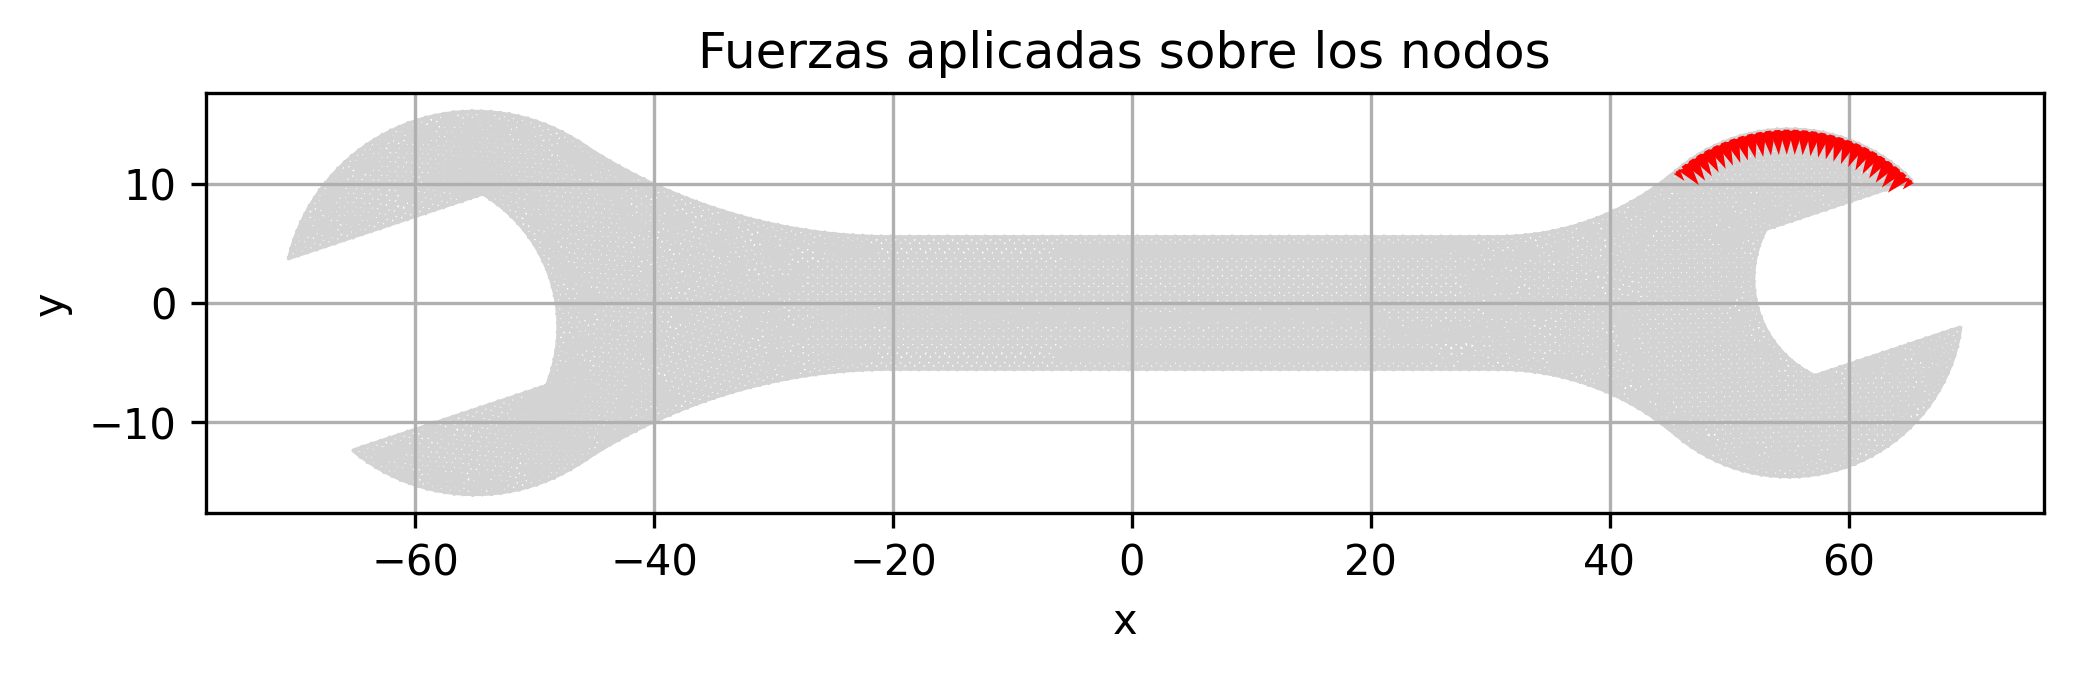
\includegraphics[width=0.8\textwidth]{GRAFICOS/Case b_fuerzas.png}
    \caption{Distributed load applied to the wrench}
    \label{fig:xd}
\end{figure}

\begin{figure}[H]
    \centering
    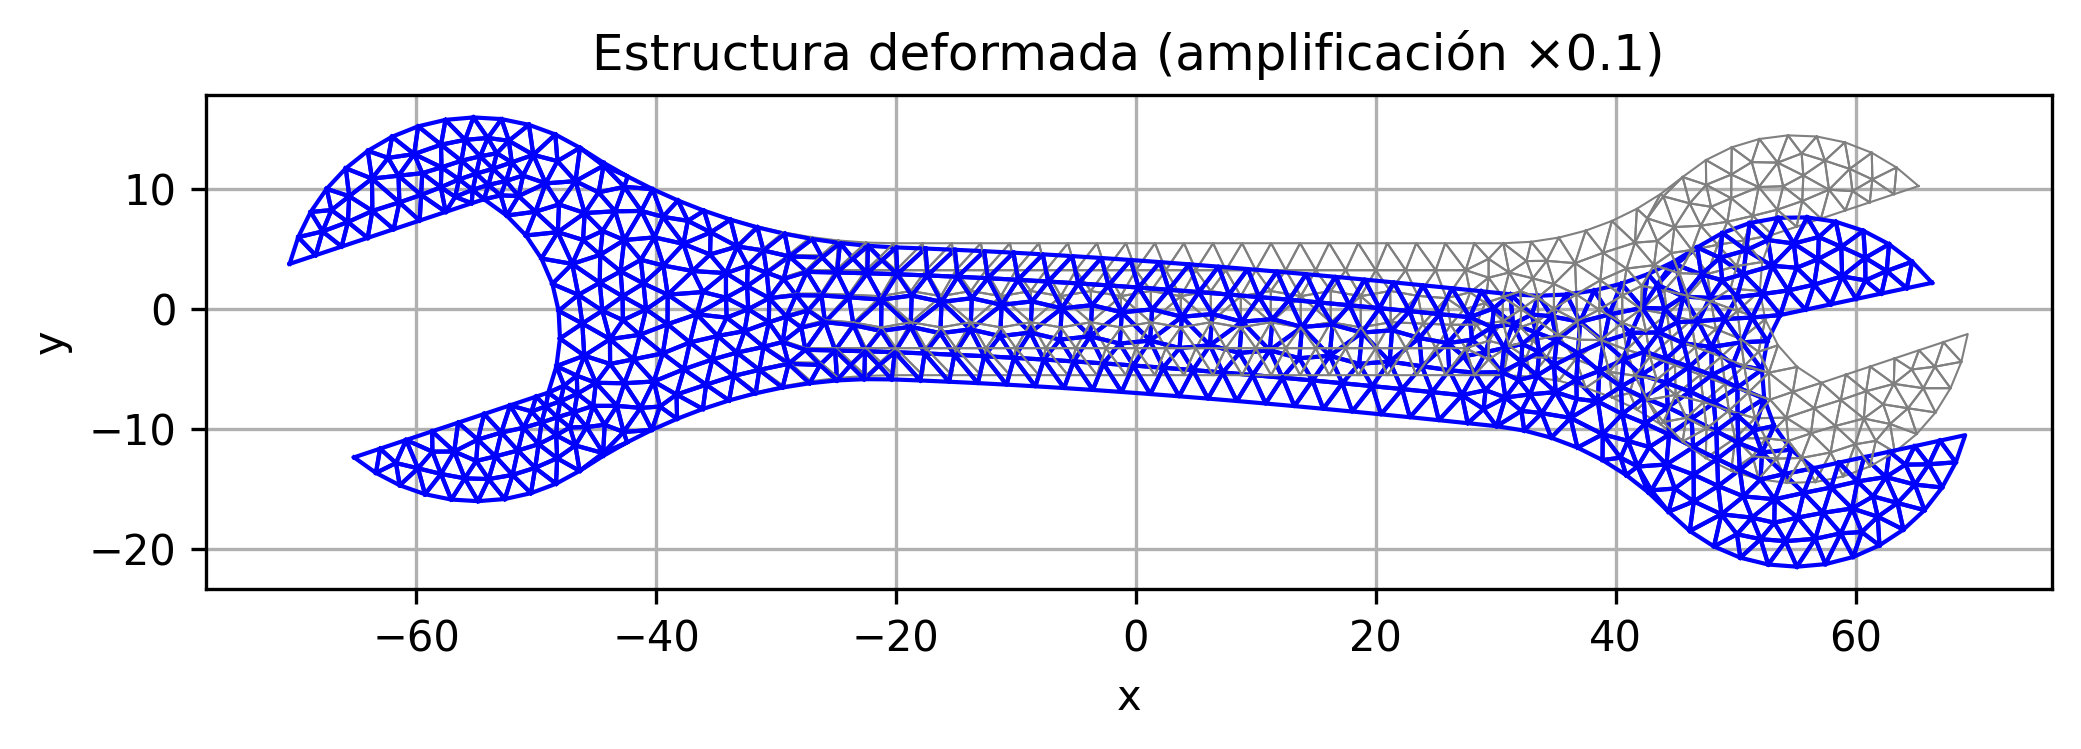
\includegraphics[width=0.8\textwidth]{GRAFICOS/Case b_deformada.png}
    \caption{Deformed wrench with distributed load}
    \label{fig:stress}
\end{figure}

The results of normal stresses, shear stresses, and displacements are shown below, as well as the principal stresses and strains.

\begin{table}[H]
    \centering
    \caption{Stress (Pa) and strain components}
    \begin{tabular}{|c|c|c|c|c|c|}
    \hline
    $\sigma_{xx}$ & $\sigma_{yy}$ & $\tau_{xy}$ & $\epsilon_{xx}$ & $\epsilon_{yy}$ & $\gamma_{xy}$ \\
    \hline
    360 & 60 & -60 & 0.09 & 0.036 & -0.05 \\
    \hline
    \end{tabular}
    \label{tab:tabla1}
\end{table}
    
\begin{table}[H]
    \centering
    \caption{Principal Stresses (Pa) and strain components}
    \begin{tabular}{|c|c|c|c|}
    \hline
    $\sigma_{1}$ & $\sigma_{2}$ & $\epsilon_{1}$ & $\epsilon_{2}$ \\
    \hline
    360 & -360 & 0.108 & -0.108 \\
    \hline
    \end{tabular}
    \label{tab:tabla2}
\end{table}

Finally, the Von Misses stress is plotted below, reaching a maximum value of $\sigma_{VM} = 360 Pa$.

\begin{figure}[H]
    \centering
    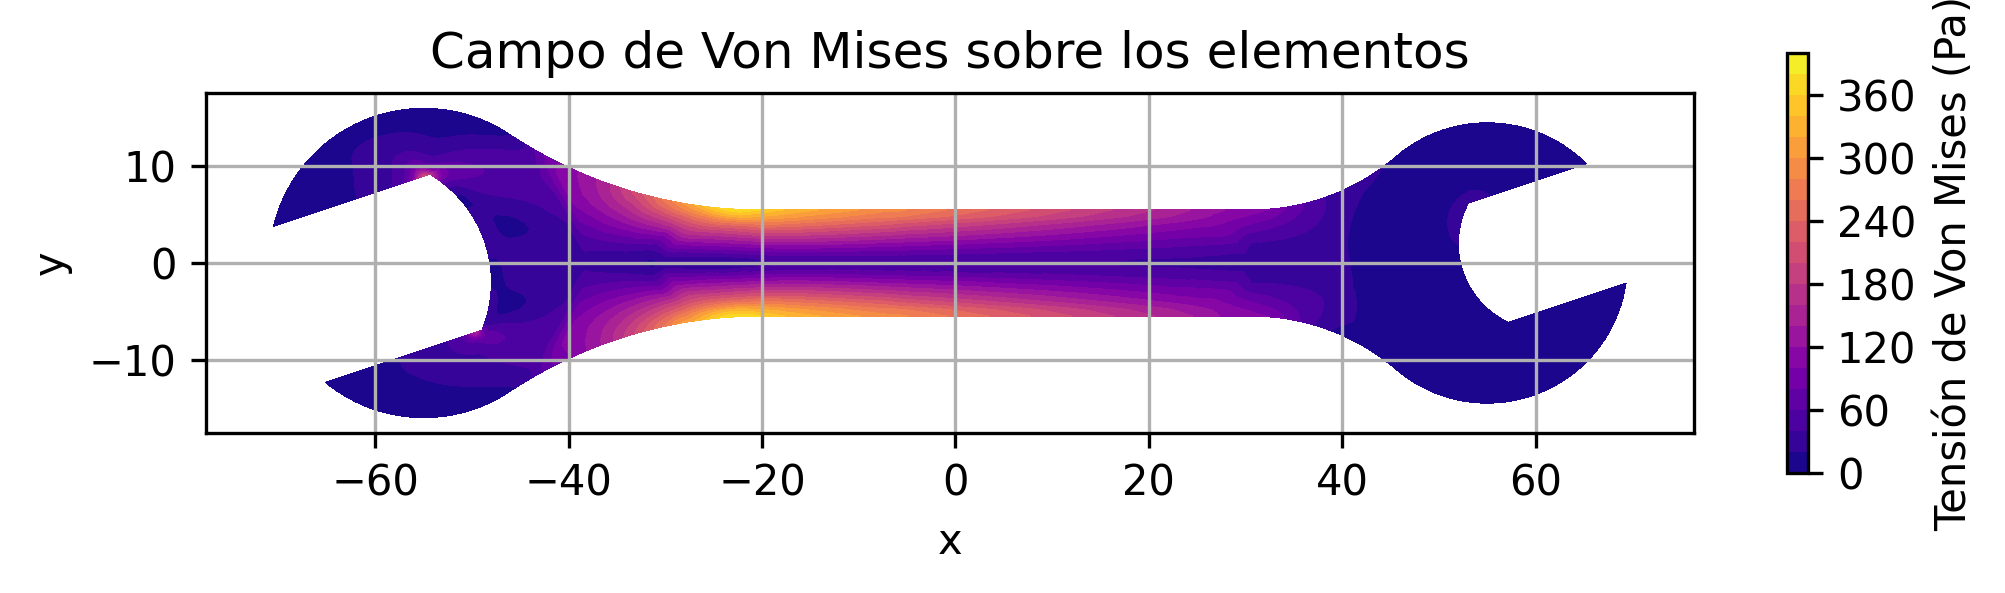
\includegraphics[width=0.8\textwidth]{GRAFICOS/Case b_von_mises.png}
    \caption{Von Misses stress distribution for the distributed load}
    \label{fig:principal}
\end{figure}

\subsection{Case 2: Point load applied to one end of the wrench}

Different to the previous case, a point load of $30 kgf$ was applied to one end of the wrench. This can be observed in Figure \ref{fig:xdd}. Also, the deformed state is shown in Figure \ref{fig:xdi}.

\begin{figure}[H]
    \centering
    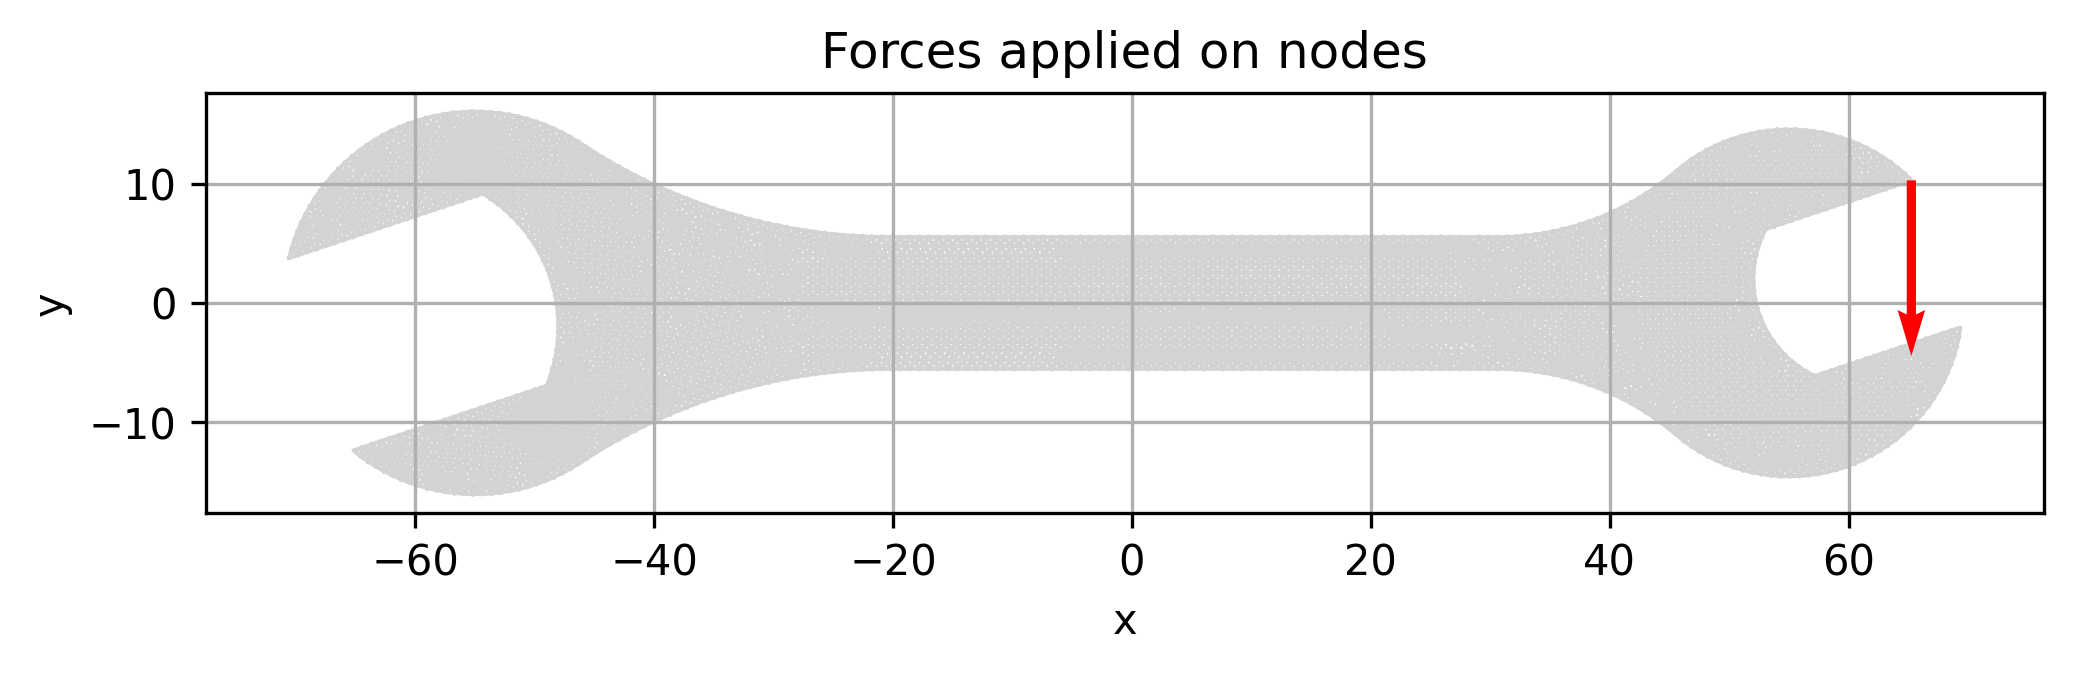
\includegraphics[width=0.8\textwidth]{GRAFICOS/Case a_fuerzas.png}
    \caption{Point load applied to the wrench}
    \label{fig:xdd}
\end{figure}

\begin{figure}[H]
    \centering
    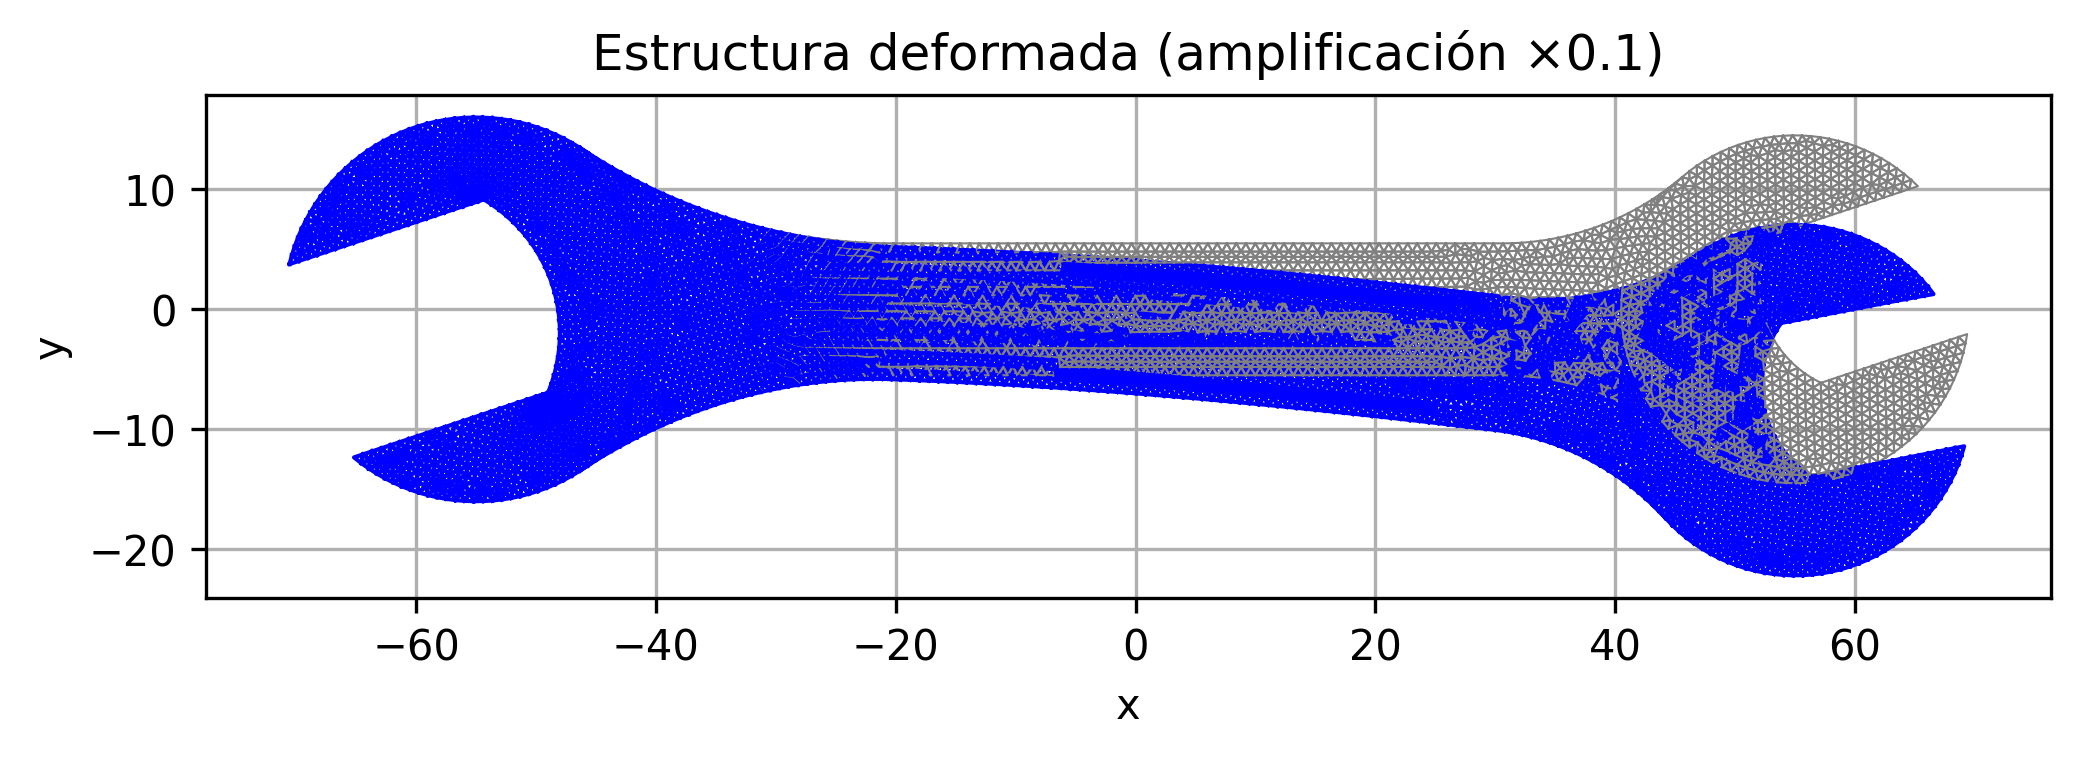
\includegraphics[width=0.8\textwidth]{GRAFICOS/Case a_deformada.png}
    \caption{Deformed wrench with point load}
    \label{fig:xdi}
\end{figure}

In the following tables, the stress and strain components are shown.

\begin{table}[H]
    \centering
    \caption{Stress (Pa) and strain components}
    \begin{tabular}{|c|c|c|c|c|c|}
    \hline
    $\sigma_{xx}$ & $\sigma_{yy}$ & $\tau_{xy}$ & $\epsilon_{xx}$ & $\epsilon_{yy}$ & $\gamma_{xy}$ \\
    \hline
    450 & 72 & -120 & 0.12 & 0.045 & -0.096 \\
    \hline
    \end{tabular}
    \label{tab:tabla1}
\end{table}
    
\begin{table}[H]
    \centering
    \caption{Principal Stresses (Pa) and strain components}
    \begin{tabular}{|c|c|c|c|}
    \hline
    $\sigma_{1}$ & $\sigma_{2}$ & $\epsilon_{1}$ & $\epsilon_{2}$ \\
    \hline
    450 & -450 & 0.128 & -0.128 \\
    \hline
    \end{tabular}
    \label{tab:tabla2}
\end{table}


It is noticeable that, compared to the previous case, the principal strains are significally higher. This is due to the fact that considering the type of material and its mechanical properties, the force magnitude and single point of application increases the stress concentration throughout the wrench. This is also reflected in the Von Misses stress, which reaches a maximum value of $\sigma_{VM} = 450 Pa$.

\begin{figure}[H]
    \centering
    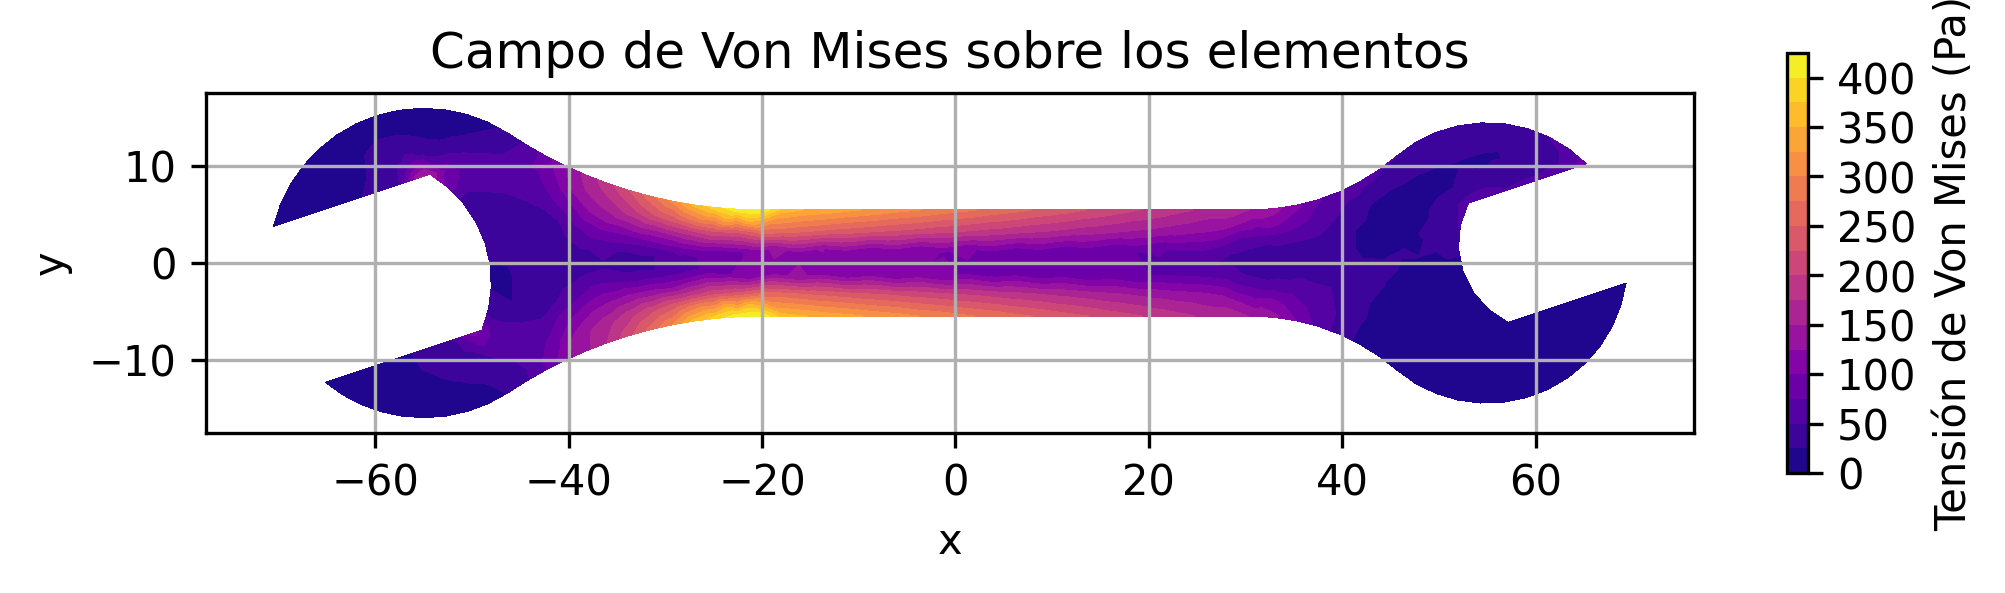
\includegraphics[width=0.8\textwidth]{GRAFICOS/Case a_von_mises.png}
    \caption{Von Misses stress distribution for the point load}
    \label{fig:principal}
\end{figure}

\subsection{Case 3: Self-weight added to the distributed load}

Now, a similar case to the first one was analyzed, but this time the self-weight was added as a body force ($m_{wrench} = 8 gr$). The results are shown below.

\begin{figure}[H]
    \centering
    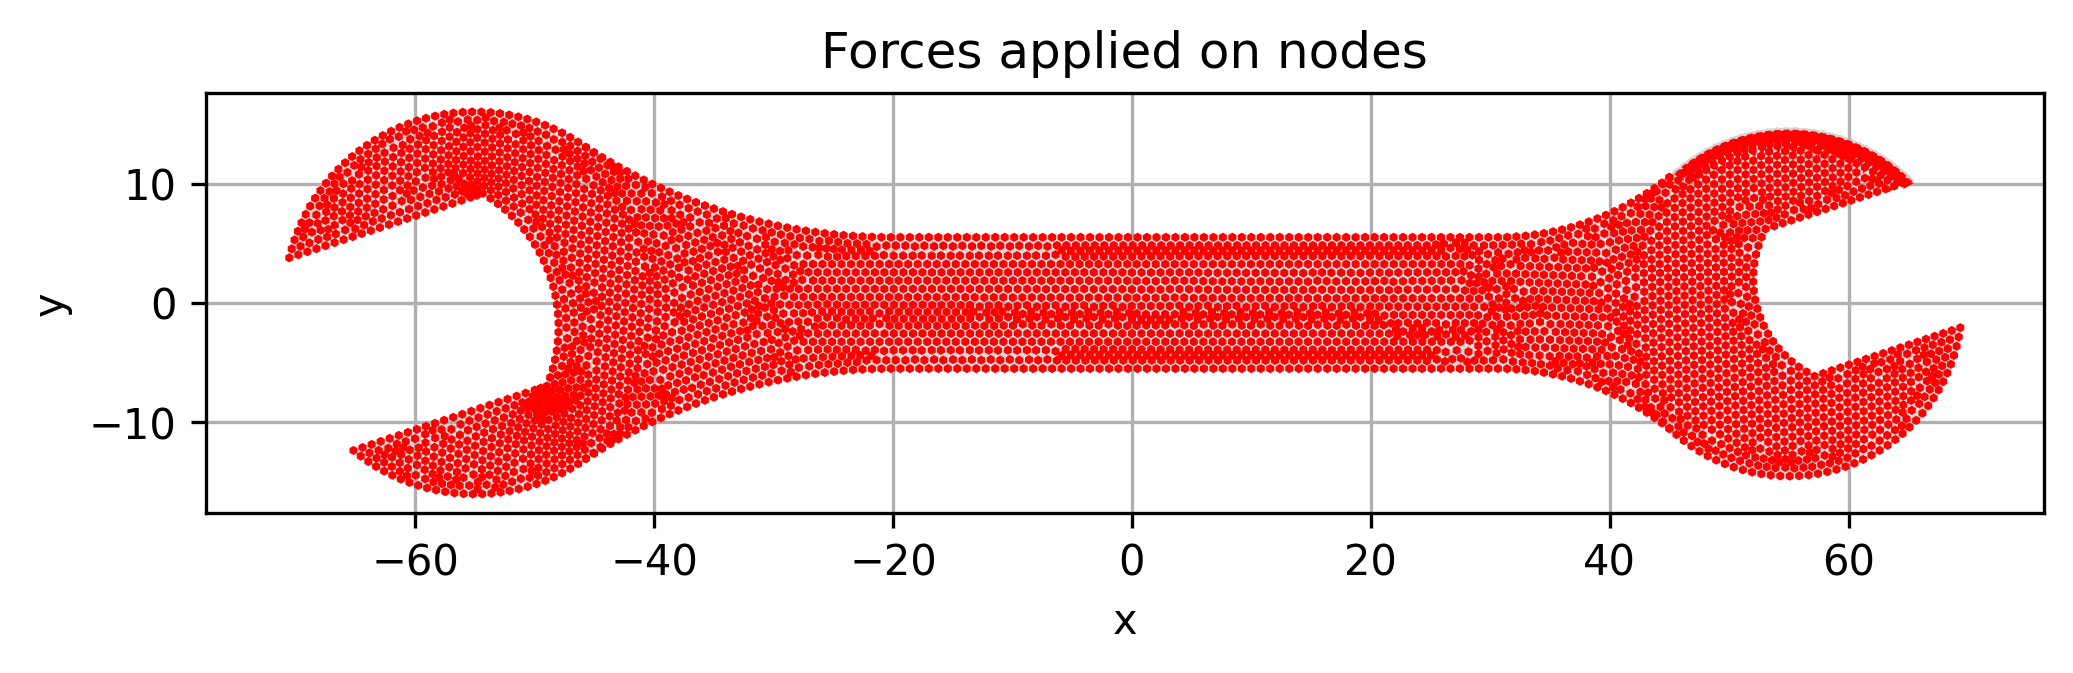
\includegraphics[width=0.8\textwidth]{GRAFICOS/Case c_fuerzas.png}
    \caption{Applied self-weight forces acting on each CST element's centroid.}
    \label{fig:xdiwi}
\end{figure}

We can observe in Figure \ref{fig:xdiwi} that the self-weight vector acts across the entire body of the wrench, specifically at the mass centroid of each CST element.  
The deformed state of the structure is shown in Figure \ref{fig:xdiwi2}.

\begin{figure}[H]
    \centering
    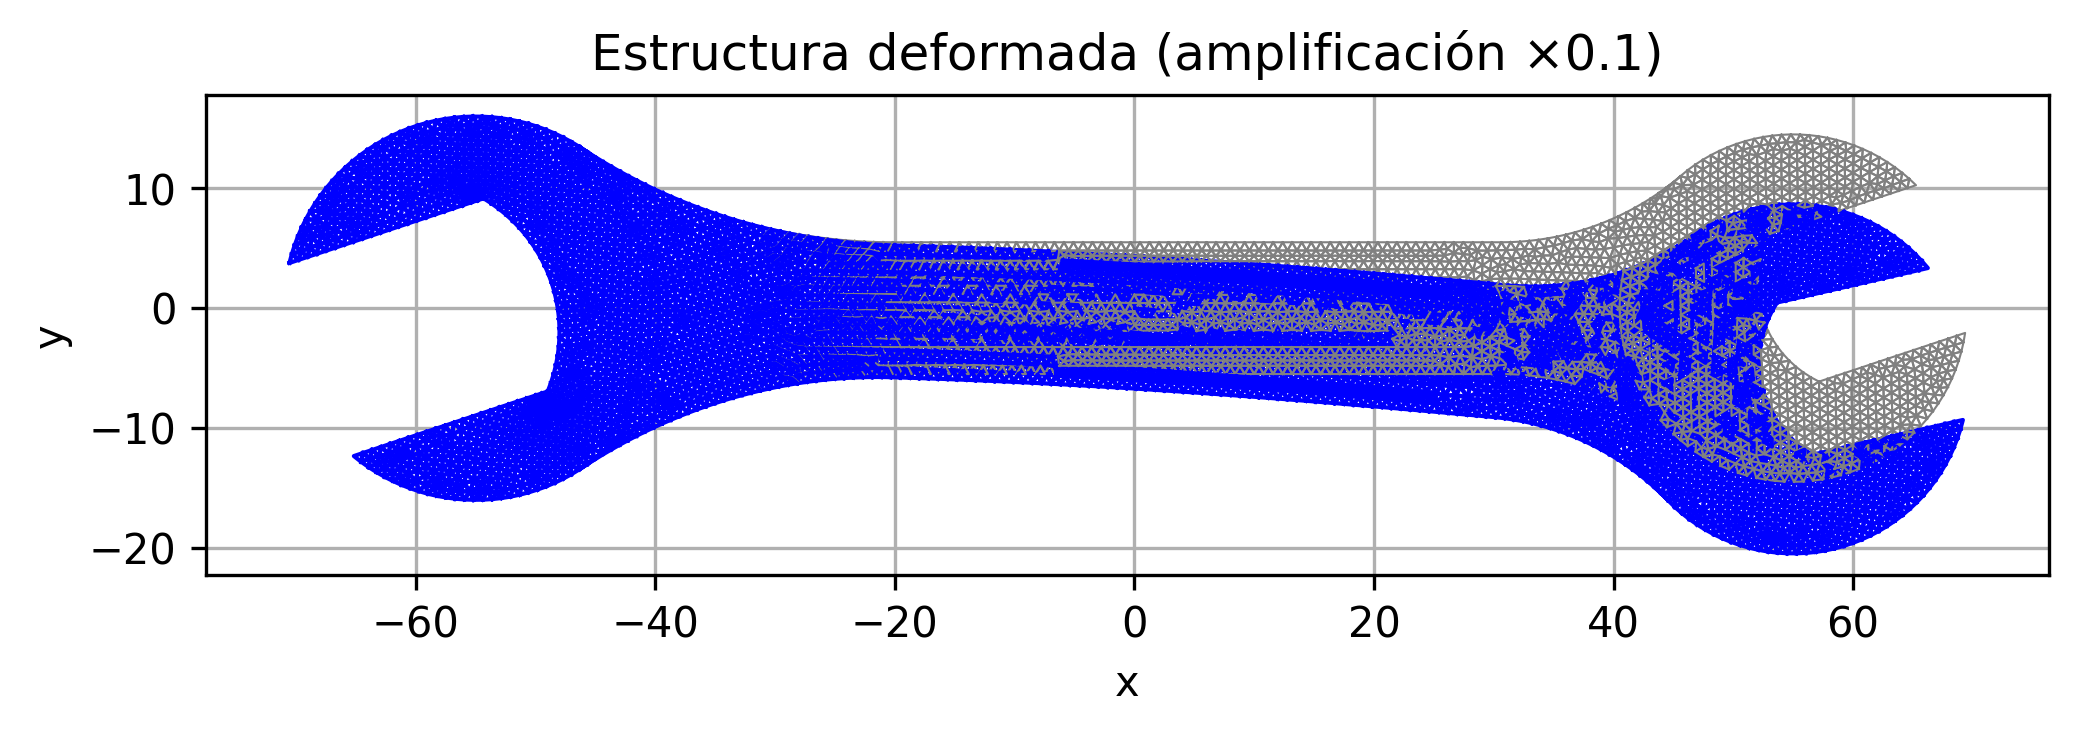
\includegraphics[width=0.8\textwidth]{GRAFICOS/Case c_deformada.png}
    \caption{Deformed configuration of the wrench under self-weight loading.}
    \label{fig:xdiwi2}
\end{figure}


\begin{table}[H]
    \centering
    \caption{Stress (Pa) and strain components}
    \begin{tabular}{|c|c|c|c|c|c|}
    \hline
    $\sigma_{xx}$ & $\sigma_{yy}$ & $\tau_{xy}$ & $\epsilon_{xx}$ & $\epsilon_{yy}$ & $\gamma_{xy}$ \\
    \hline
    360 & 60 & -60 & 0.09 & 0.036 & -0.05 \\
    \hline
    \end{tabular}
    \label{tab:tabla1}
\end{table}
    
\begin{table}[H]
    \centering
    \caption{Principal Stresses (Pa) and strain components}
    \begin{tabular}{|c|c|c|c|}
    \hline
    $\sigma_{1}$ & $\sigma_{2}$ & $\epsilon_{1}$ & $\epsilon_{2}$ \\
    \hline
    360 & -360 & 0.108 & -0.108 \\
    \hline
    \end{tabular}
    \label{tab:tabla2}
\end{table}

Comparing this scenario with the one presented in Case 1, the results are the same. This is because the self-weight of the wrench is negligible compared to the distributed load of $30 kgf$. Therefore, the internal stresses and strains are not affectedd by it.

\subsection{Case 4: Only self-weight applied as a body force}

The decision to analyze this singular case was made in order to observe and compere how this body force condition affected the wrench. This way, we can observe that, due to the conditions of restrcited nodes in one end, the wrench still deforms, but in a much smaller magnitude.

\begin{figure}[H]
    \centering
    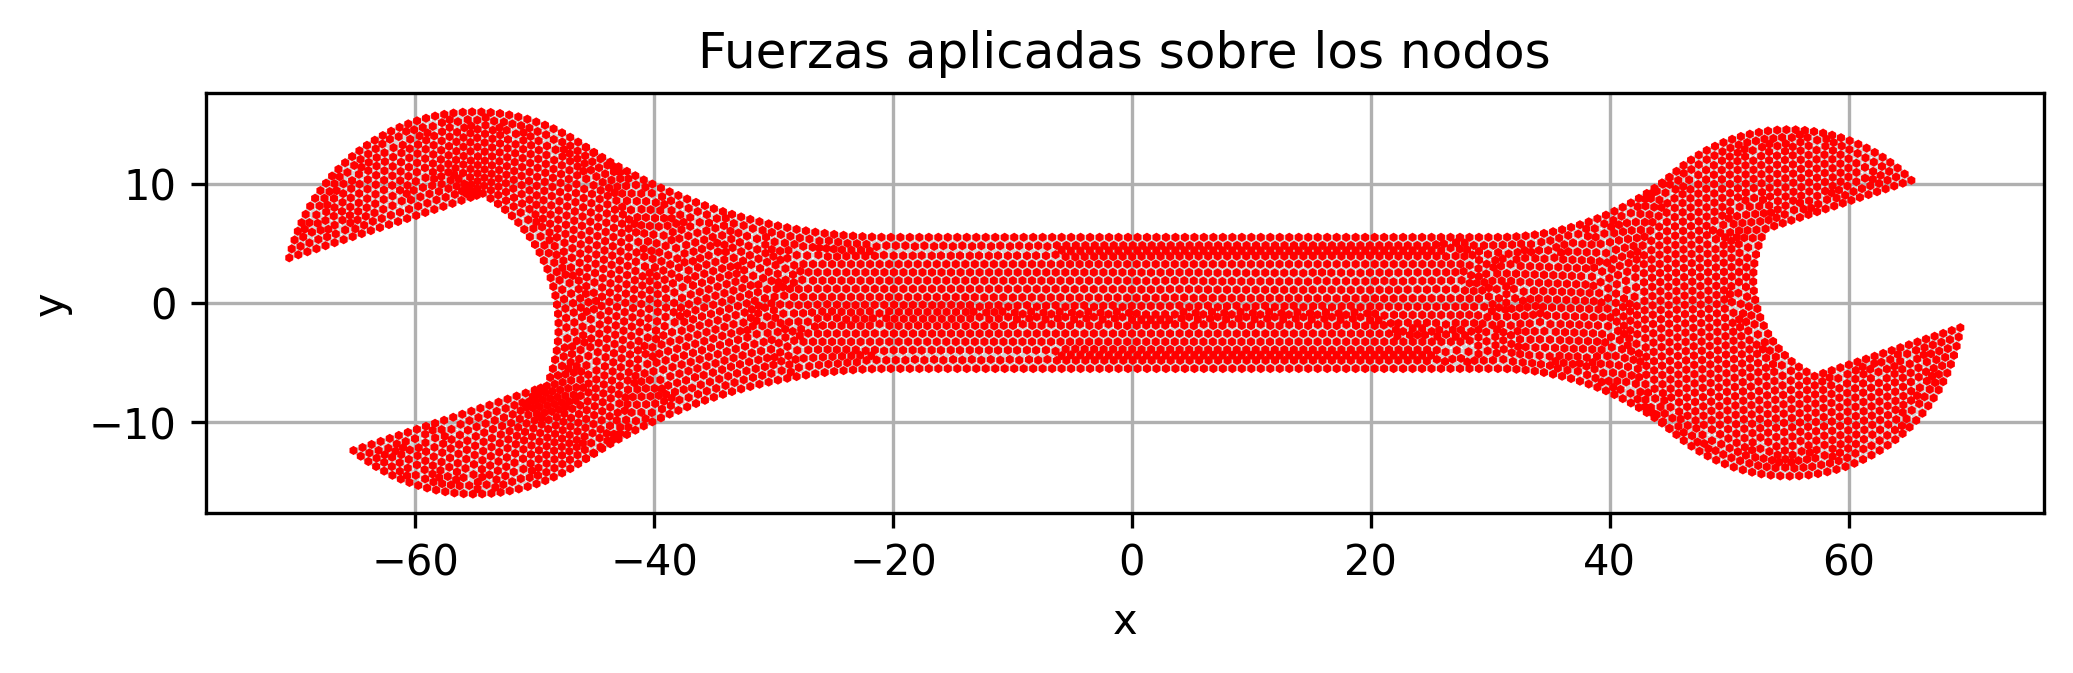
\includegraphics[width=0.8\textwidth]{GRAFICOS/Case d_fuerzas.png}
    \caption{Self-weight applied as a body force}
    \label{fig:bf}
\end{figure}

\begin{figure}[H]
    \centering
    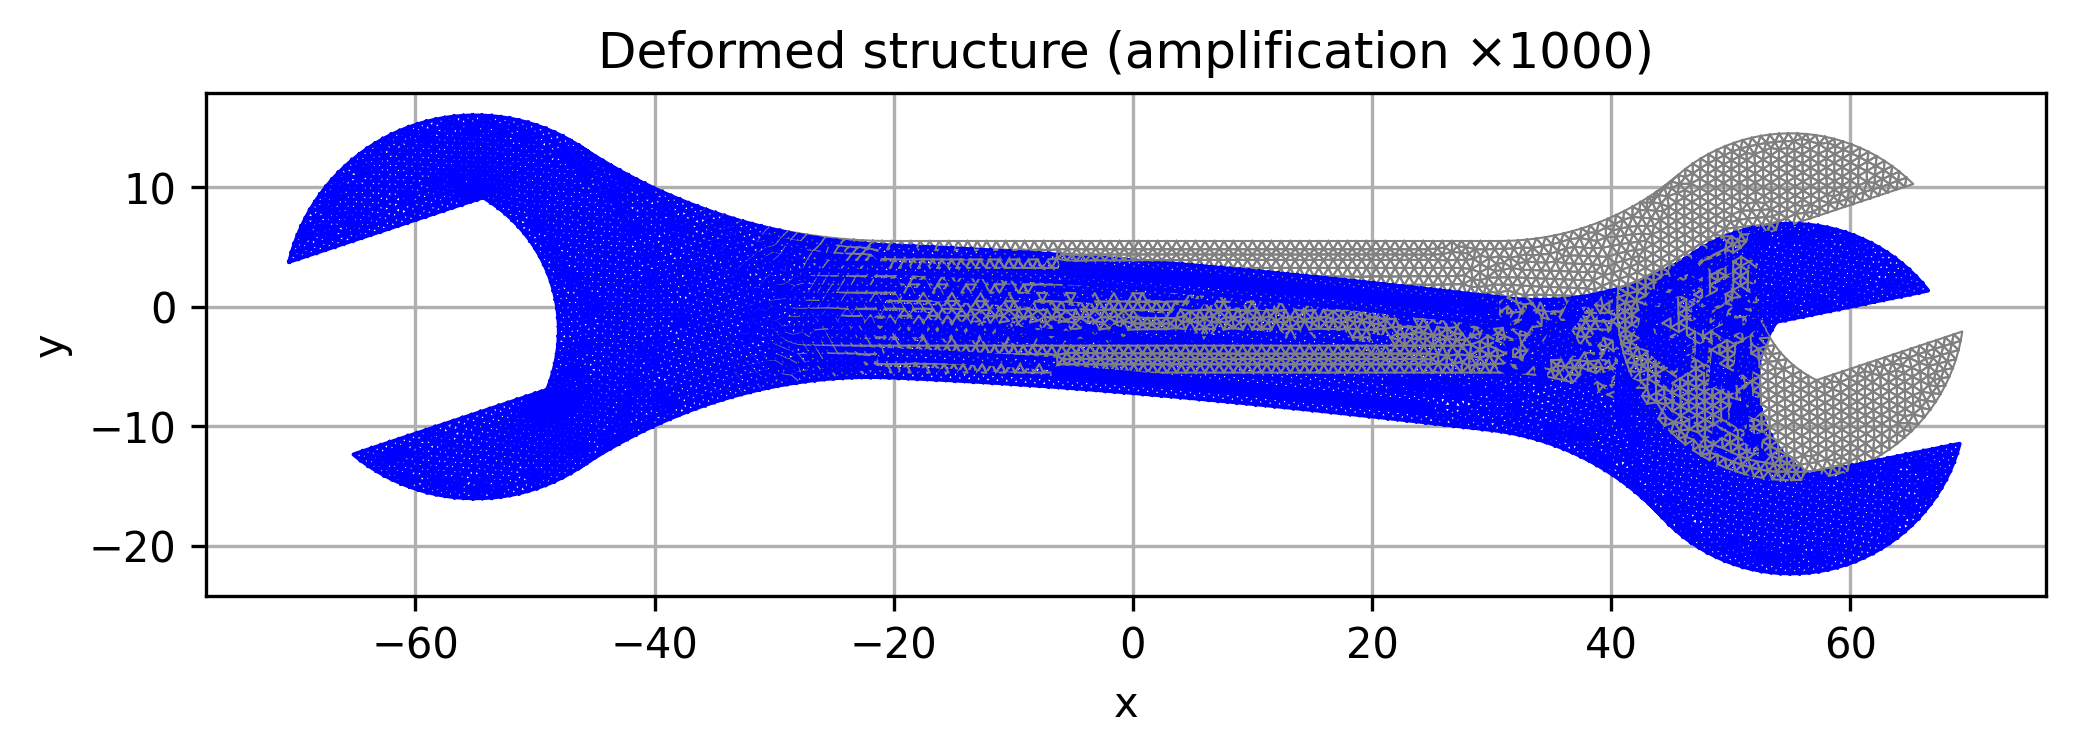
\includegraphics[width=0.8\textwidth]{GRAFICOS/Case d_deformada.png}
    \caption{Deformed wrench with self-weight}
    \label{fig:bf1}
\end{figure}

Notice the amplification factor of the deformed state, which is $10^3$. Which is a clear indication of the small magnitude of the displacements compared to the previous 3 cases. The stress and strain components are shown below.

\begin{table}[H]
    \centering
    \caption{Stress (Pa) and strain components}
    \begin{tabular}{|c|c|c|c|c|c|}
    \hline
    $\sigma_{xx}$ & $\sigma_{yy}$ & $\tau_{xy}$ & $\epsilon_{xx}$ & $\epsilon_{yy}$ & $\gamma_{xy}$ \\
    \hline
    0.045 & 0.012 & -0.0096 & $1.35\times10^{-5}$ & $4.5\times10^{-6}$ & $6.4\times10^{-6}$ \\
    \hline
    \end{tabular}
    \label{tab:tabla1}
\end{table}
    
\begin{table}[H]
    \centering
    \caption{Principal Stresses (Pa) and strain components}
    \begin{tabular}{|c|c|c|c|}
    \hline
    $\sigma_{1}$ & $\sigma_{2}$ & $\epsilon_{1}$ & $\epsilon_{2}$ \\
    \hline
    0.048 & -0.0525 & $1.44\times10^{-5}$ & $-1.44\times10^{-5}$ \\
    \hline
    \end{tabular}
    \label{tab:tabla2}
\end{table}

Observing the plot of the Von Mises stresses, we can see that the maximum value is $\sigma_{VM} = 0.0525\ \text{Pa}$.  
This clearly indicates the low impact of the self-weight on the wrench structure.

\begin{figure}[H]
    \centering
    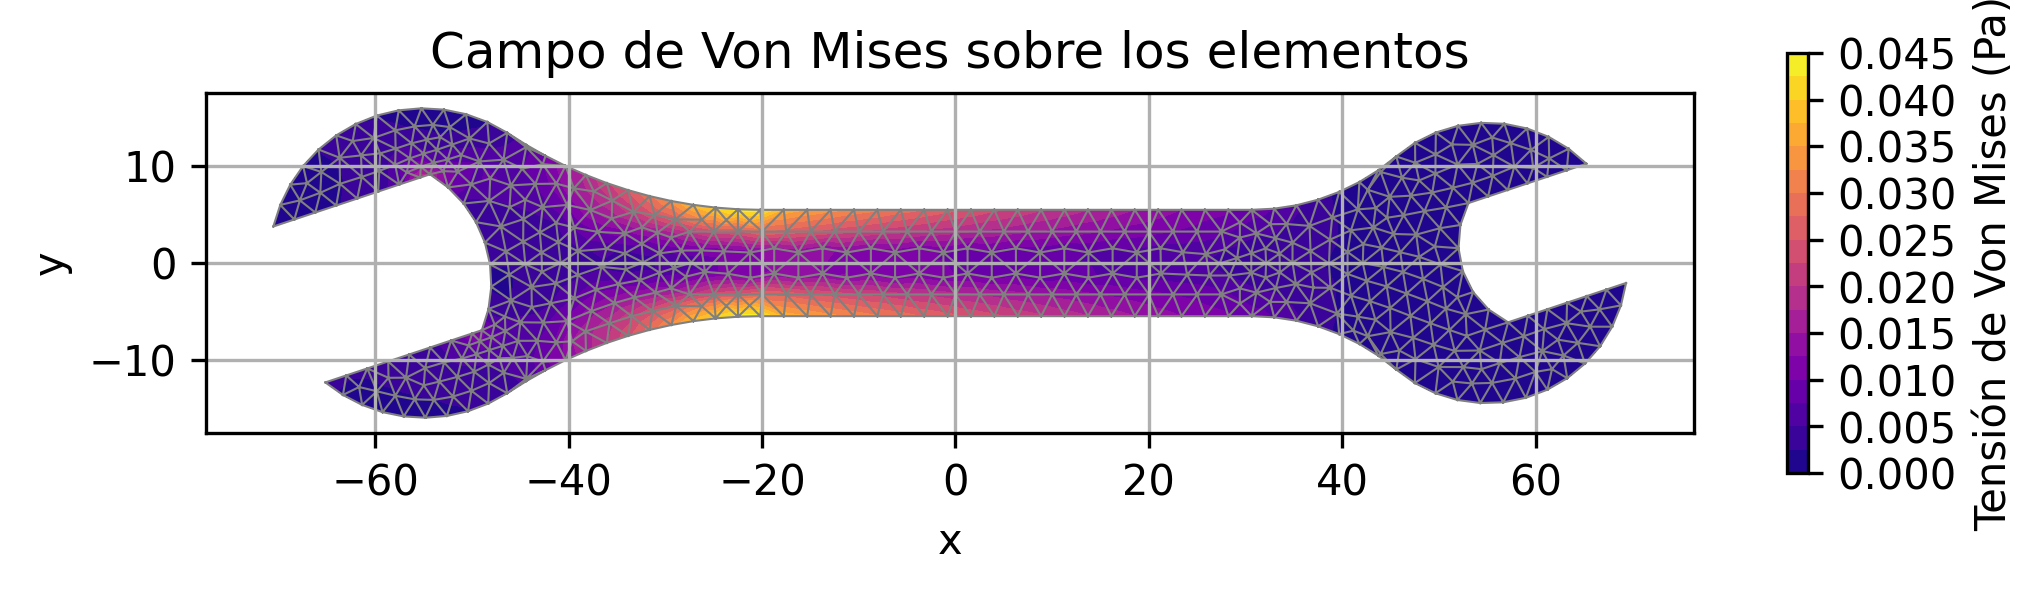
\includegraphics[width=0.8\textwidth]{GRAFICOS/Case d_von_mises.png}
    \caption{Von Mises stress distribution under self-weight loading.}
    \label{fig:principal}
\end{figure}


Finally, the simulation shows the clear mechanical behavior of the PLA wrench under different loading conditions. Where the CST model was able to capture accuratly and with precision the internal stresses and strains of the element. The results were coherent with the physical behavior of it, and the Von Misses stress was able to capture the stress concentration in the areas of interest. The results were also consistent with the expected behavior of a wrench under different loading conditions.




